\documentclass{scrartcl}

\usepackage[T1]{fontenc}
\usepackage[utf8]{inputenc}
\usepackage[ngerman]{babel}
\usepackage{tgheros}
\renewcommand{\familydefault}{\sfdefault}

\usepackage[margin=0cm]{geometry}
\usepackage[hidelinks]{hyperref}

\usepackage{tikz}
\usetikzlibrary{calc,shadows,decorations.text}

\usepackage{graphicx}
\usepackage{xcolor}

\definecolor{fsfw-cyan}{HTML}{28ADB8}
\definecolor{fsfw-violett}{HTML}{654BC7}
\definecolor{fsfw-green}{HTML}{6BBB00}

\begin{document}

\begin{tikzpicture}[overlay,remember picture]
  
  % background
  \foreach \i in {-1,0,1,2,3,4,5} {
    \node[anchor=north,overlay] at ($(current page.north) + 5.65*(0,-\i)$) {
      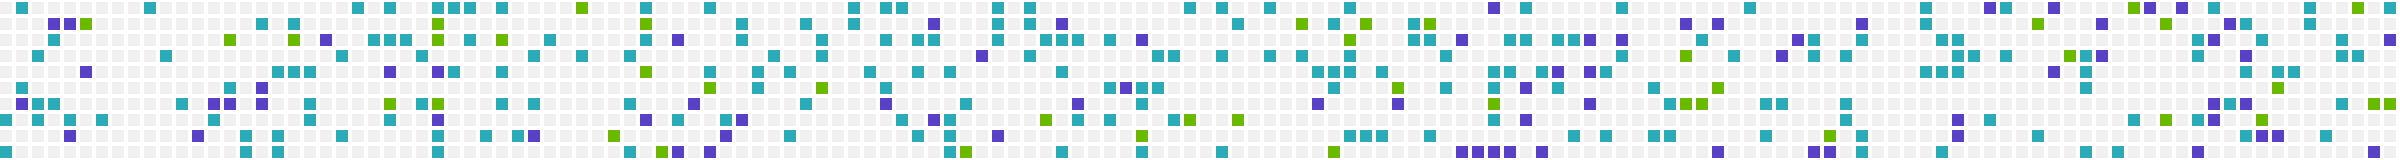
\includegraphics{banner.png}
    };
  }
  
  % top
  \node[anchor=north,fill=white,rounded corners=1cm]
  at ($(current page.north) + (0,-1)$)
  {
    \begin{tikzpicture}
      \useasboundingbox (-9,5) rectangle (9,-5);
      \node[scale=3,at={(-3,4)},color=fsfw-cyan]{\textbf{\Huge\LaTeX?}};
      \node[scale=3,at={( 3,-1)},color=fsfw-violett]{\textbf{\Huge Hilfe!}};
      \begin{scope}[every node/.style={scale=1.5}]
        \node[at={(-7,0)}]{\Large Poster};
        \node[at={(-4.5,-2)}]{\Large Abschlussarbeit};
        \node[at={(4,1)}]{\Large Präsentation};
        \node[at={(6,3)}]{\Large Seminararbeit};
      \end{scope}
      \draw[ rounded corners=0cm, decoration={
        reverse path,
        text along path,
        text={}}]
      (0,0)
      \foreach \i [evaluate={\r=(\i/2000)^2;}] in {0,5,...,5000}{ -- (\i:\r)}; 
    \end{tikzpicture}
  };


  % middle
  \node[fill=white,rounded corners=1cm] at ($(current page.center) + (0,-3.4)$){
    \begin{tikzpicture}
      \useasboundingbox (-9,6) rectangle (9,-6);
    \end{tikzpicture}
  };
  
  % footer
  \node[anchor=south,fill=white,rounded corners=1cm]
  at ($(current page.south) + (0,0.5)$) {
    \begin{tikzpicture}
      \useasboundingbox (-9,2) rectangle (9,-2);
      \node[rectangle,minimum height=3.5cm,minimum width=19cm] at (0,-2){
        \parbox[b][3.5cm]{4.5cm}{
          \null\vfill\centering
          
\includegraphics[origin=cc,width=4cm]{sitelogo.png}
          \vfill\null
        }
        \parbox[b][3.5cm]{13.5cm}{
          \null\vfill
          \centering
          \LARGE
          Hochschulgruppe für\\
          \Huge
          Freie Software und Freies Wissen\\
          \Large
          \medskip
          \url{https://fsfw-dresden.de}
          \vfill\null
        }
      };
    \end{tikzpicture}
  };
\end{tikzpicture}

\newpage

\end{document}

%%% Local Variables:
%%% mode: latex
%%% TeX-master: t
%%% End:
